\subsection{Wirksamkeit von Shift-Left Maßnahmen}

In den vorherigen Textabschnitten wurde erklärt, wie Shift-Left in spezifischeren Modellen mit verschiedenen Tools umgesetzt werden kann. Um eine Einschätzung der Wirksamkeit von Shift-Left zu erhalten, wird im Folgenden ein Beitrag von \citet{andriadi_impact_2023} betrachtet.

\begin{figure}
\centering
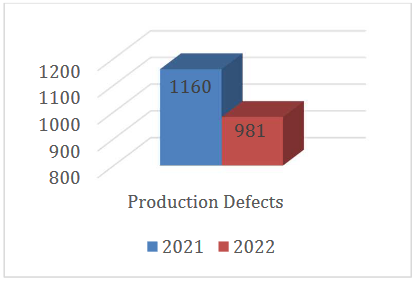
\includegraphics[width=0.9\linewidth]{images/Impact_production_defects.png}
\caption{Diagramm zur Menge an Fehlern im Jahr 2021 und 2022 aus \cite{andriadi_impact_2023}}
\label{fig:production_defects }
\end{figure}

\citet{andriadi_impact_2023} untersuchten dafür die Menge an Fehlern in einem indonesischen Tech-Unternehmen in den Jahren 2021 und 2022. Das Unternehmen entwickelte zunächst ein Jahr ohne den Shift-Left-Ansatz und im darauffolgenden Jahr mit dem Shift-Left-Ansatz. Die Änderungen, die das Unternehmen 2022 vornahm, beinhalteten hauptsächlich die Arbeitsweise und die Rolle der Entwickler sowie der QA-Teams:
\begin{enumerate}
\item Tests werden bereits in der Entwicklungsphase geschrieben und nicht nur in einer gesonderten Testphase.
\item Entwickler schreiben Basis-Tests für ihre eigenen Features und beheben dadurch entdeckte Fehler eigenständig.
\item QA erstellt parallel automatisierte Testskripte für den aktuellen Sprint. Die Menge der manuellen Tests wurde reduziert und mehr automatisierte Tests geschrieben.
\item Entwickler und QA halten gemeinsame tägliche Meetings, um Testanforderungen zu klären. Alle gefundenen Fehler werden dokumentiert und kategorisiert.
\end{enumerate}

In Abbildung \ref{fig:production_defects } ist die Menge der Produktionsfehler in beiden Jahren zu erkennen. Dabei ist festzustellen, dass die Menge an gefundenen Fehlern von 1160 auf 981 gesunken ist. Dies entspricht einer Reduzierung von etwa 15\%. Diese Verbesserung wird durch die frühere Erkennung von Fehlern in der Entwicklungsphase begründet, da das Projekt dort weniger Quellcode und Komplexität aufweist \cite{andriadi_impact_2023}. Ebenfalls konnten die Fehler bei Regressionstests um 24\% und bei Integrationstests um 57\% reduziert werden. Diese Metriken zeigen, dass der Shift-Left-Ansatz dazu beitragen kann, spätere Kosten zu reduzieren. Der gesamte Prozess brachte jedoch auch Herausforderungen mit sich: Die Entwickler benötigten mehr Zeit, da sie zusätzlich Tests schreiben mussten, und der Entwicklungsprozess war abhängig von einer gut funktionierenden Kommunikation \cite{andriadi_impact_2023}. Die Ergebnisse zeigen zwar, dass sich dieser Mehraufwand langfristig ausgleicht, dennoch muss der Shift-Left-Ansatz konsequent umgesetzt werden.

Die in der Studie demonstrierte Wirksamkeit von Shift-Left Testing lässt sich analog auf Shift-Left-Security übertragen. Indem Sicherheitsprüfungen bereits in den frühen Entwicklungsphasen integriert werden, lassen sich Risiken minimieren und somit Kosten senken. Die vorgestellte Studie unterstützt dies indirekt, da sie zeigt, dass durch frühzeitige Qualitätssicherung kritische Defekte verhindert werden können – ein Prinzip, das sich auf Sicherheitskontexte übertragen lässt.